\section{Aproximación por Greedy}

Proponemos dos aproximaciones extra.

\subsection{Máximo por grupo}
Este enfoque realiza un cálculo de la frecuencia con la que cada jugador aparece en los $m$ subconjuntos $B$. Posteriormente, procede a recorrer cada uno de estos subconjuntos y, si la solución parcial propuesta no incluye ningún jugador presente en un subconjunto dado, se incluye en esta solución al jugador que tiene la mayor frecuencia de apariciones dentro de dicho subconjunto.

Este algorítmo sigue la técnica de diseño greedy al enfocarse en optimizar la solución global mediante la búsqueda de óptimos locales en cada subconjunto. Se prioriza la inclusión del jugador con la mayor frecuencia de aparición en situaciones donde la solución parcial no incluye a ningún jugador del subconjunto evaluado. Este método busca mejorar la solución global al introducir jugadores de acuerdo con su frecuencia de aparición en los subconjuntos, maximizando así la cobertura de conjuntos dentro de la solución propuesta.

\lstinputlisting[language=Python, firstline=1, lastline=33]{../algoritmos/greedy.py}

La primera operación tiene complejidad $O(b \times m)$, con $b$ el cardinal máximo de jugadores por subconjunto y $m$ la cantidad de subconjuntos totales. Con grupos más chicos, el algoritmo tiende a lineal ($O(m)$) y con grupos más grandes, a $O(b\times m)$. 
De la misma manera, la segunda operación tiene complejidad de  $O(b\times m)$ ya que por cada subconjunto ($O(m)$) se deben recorrer todos sus jugadores para verificar si efectivamente están en la solución final ($O(b)$) y, en caso de que no esté ninguno, se debe encontrar el jugador con máximas apariciones $O(1)$ (esta operación se va contemplando a medida que se verifica la anterior condición). De esta manera, la complejidad total es $O(2(b \times m))=O(b \times m)$ y resulta polinomial.

\subsection{Máximo global con recálculo}

La segunda estrategia inicia de manera similar, llevando a cabo el cálculo de la frecuencia de aparición de cada jugador en los diferentes subconjuntos. Posteriormente, se procede a añadir a la solución el jugador que presenta la mayor cantidad de apariciones entre todos, y quita las apariciones de los subconjuntos que ya cubre al resto de los jugadores. Este proceso se repite sucesivamente hasta quedarse sin jugadores restantes o hasta que el jugador con la mayor frecuencia encontrada no tenga más apariciones restantes.

La técnica de diseño empleada en este algoritmo, al igual que el anterior explicado, se caracteriza por ser greedy, ya que busca optimizar la solución al priorizar la inclusión del jugador con la mayor frecuencia en cada iteración, hasta alcanzar la cobertura total de todos los subconjuntos. 

\lstinputlisting[language=Python, firstline=36, lastline=69]{../algoritmos/greedy.py}

La complejidad de la primera operación es $O(b \times m)$. La complejidad de la segunda es más dificil de acotar. La iteración del \texttt{while len ( apariciones ) != 0:} se detiene cuando todos los jugadores cuentan con $0$ apariciones o recorrimos todos los jugadores. Llamaremos a esta cantidad $j \leq n$. Luego tenemos los dos \texttt{for} anidados que iteran por la cantidad de conjuntos a los que pertenece cada jugador y por todos los jugadores de cada conjunto. La primera, a la que llamaremos $g$ está acotada superiormente por la cantidad de conjuntos $m$. Luego, la segunda está acotada por $b$, el cardinal máximo de los conjuntos. Esto resultaría en una complejidad $O(n\times m\times b)$. Sin embargo, es importante notar que el único caso en que $j=n$ es cuando $b=1$, de complejidad $O(n\times m)$. A su vez, $g$ no son independientes de $b$ y $m$ ya que, cuando más grandes son los conjuntos, a más conjuntos va a pertenecer cada jugador. Así, $g \propto^{+} m$, $g \propto^{+} b$, $g \propto^{-} n$. Por esto, la complejidad nunca alcanzaría $O(n\times m\times b)$.

\section{Ejemplos}

A continuación, compararemos los resultados obtenidos por nuestras dos aproximaciones Greedy en distintos ejemplos.

El primero, ilustrado en la fig. \ref{fig:greedy_ej1}, es un caso feliz en el que los dos algoritmos obtienen el resultado óptimo.

\begin{figure}[H]
    \centering
    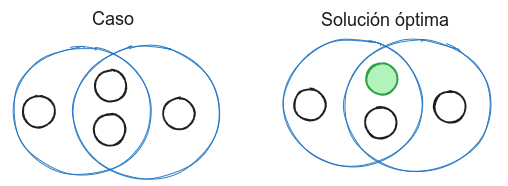
\includegraphics[width=0.8\textwidth]{img/greedy_ej1.png}
    \caption{Ejemplo 1}
    \label{fig:greedy_ej1}
\end{figure}

\begin{figure}[H]
    \centering
    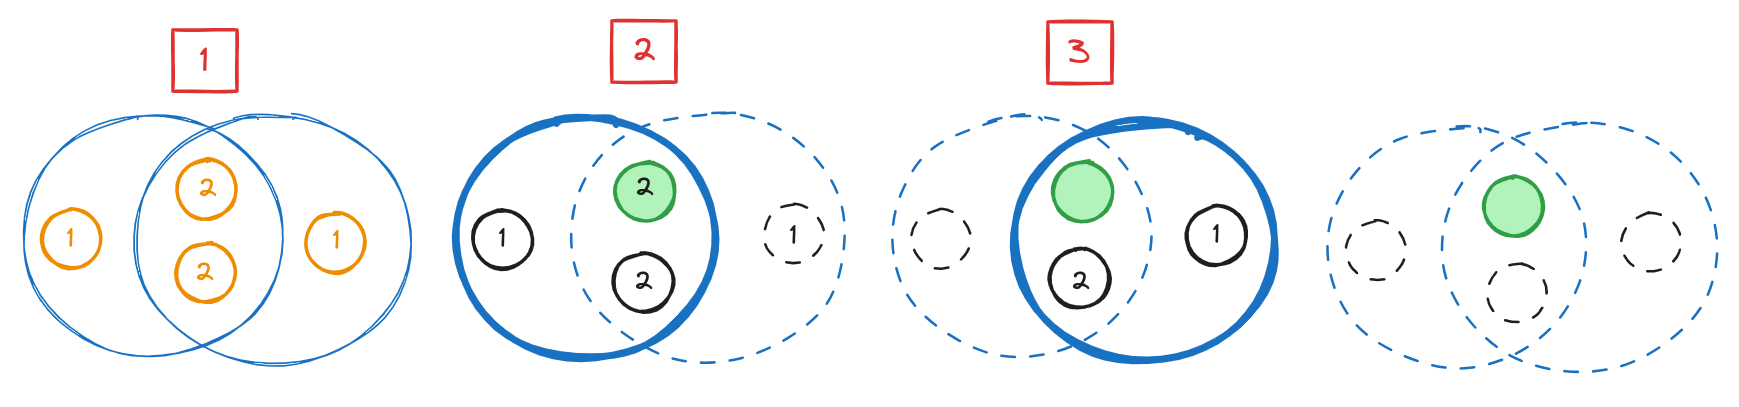
\includegraphics[width=0.8\textwidth]{img/greedy_ej1_mpg.png}
    \caption{Ejemplo 1 resuelto por Máximo por grupo}
    \label{fig:greedy_ej1_mpg}
\end{figure}

\begin{figure}[H]
    \centering
    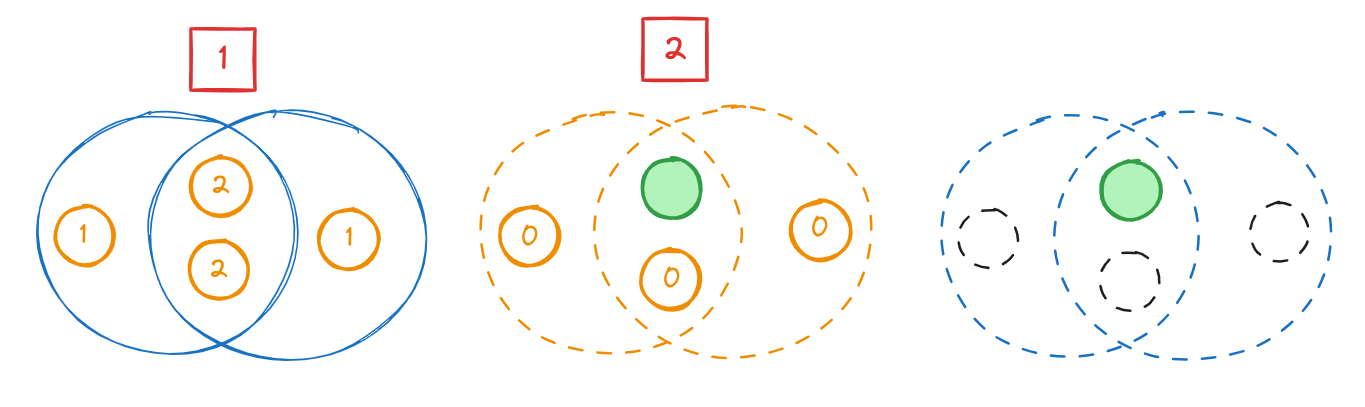
\includegraphics[width=0.8\textwidth]{img/greedy_ej1_mgr.png}
    \caption{Ejemplo 1 resuelto por Máximo global con recálculo}
    \label{fig:greedy_ej1_mgr}
\end{figure}

El segundo ejemplo (fig. \ref{fig:greedy_ej2}) podemos observar en la fig. \ref{fig:greedy_ej2_mpg} que "Máximo por grupo", de menor complejidad, no encuentra la solución óptima, pero el "Máximo global con recálculo", en la fig. \ref{fig:greedy_ej2_mgr}, si.

\begin{figure}[H]
    \centering
    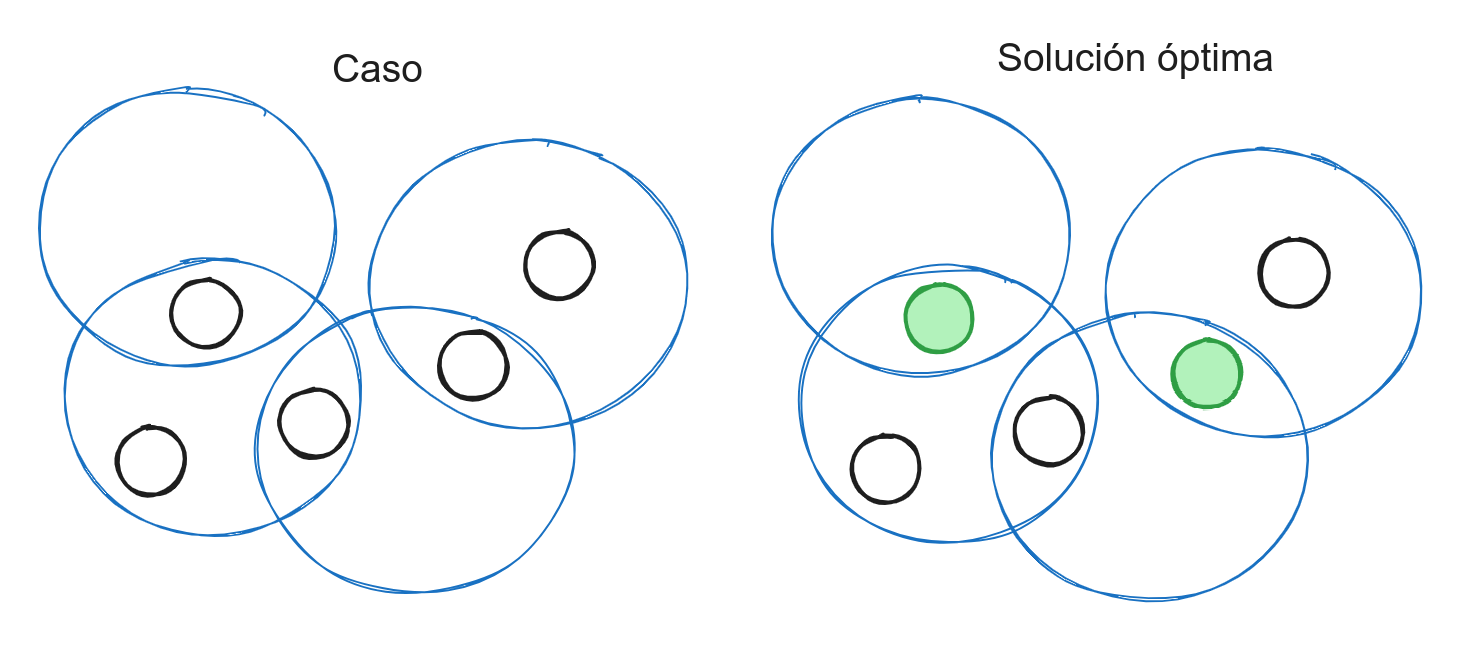
\includegraphics[width=0.8\textwidth]{img/greedy_ej2.png}
    \caption{Ejemplo 2}
    \label{fig:greedy_ej2}
\end{figure}

\begin{figure}[H]
    \centering
    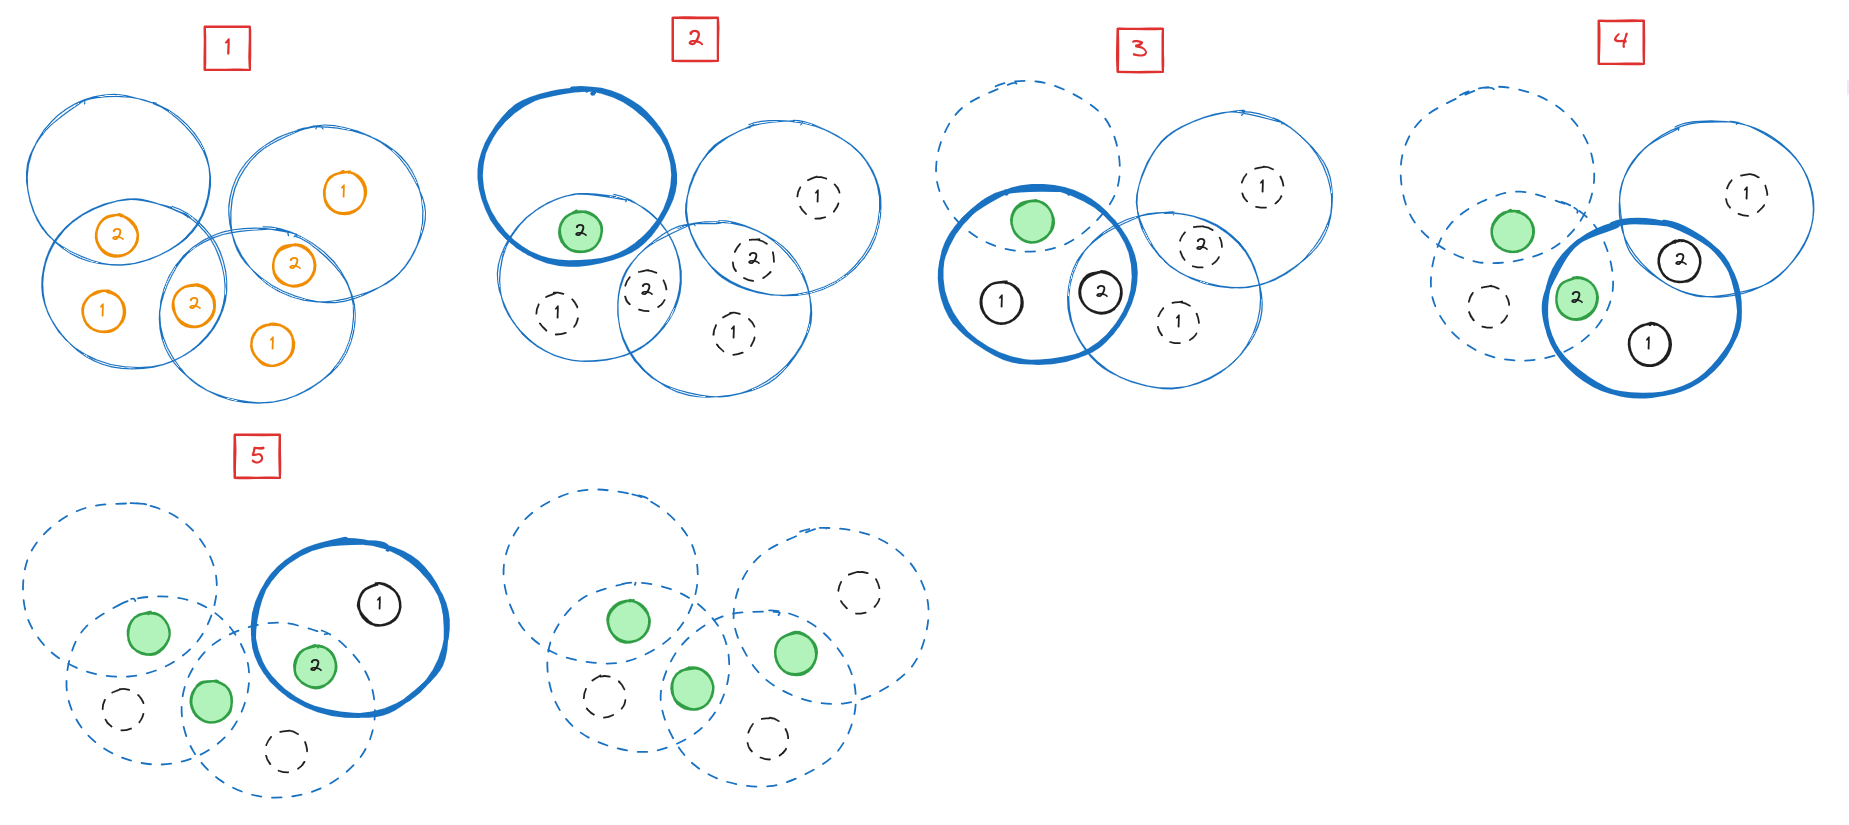
\includegraphics[width=0.8\textwidth]{img/greedy_ej2_mpg.png}
    \caption{Ejemplo 2 resuelto por Máximo por grupo}
    \label{fig:greedy_ej2_mpg}
\end{figure}

\begin{figure}[H]
    \centering
    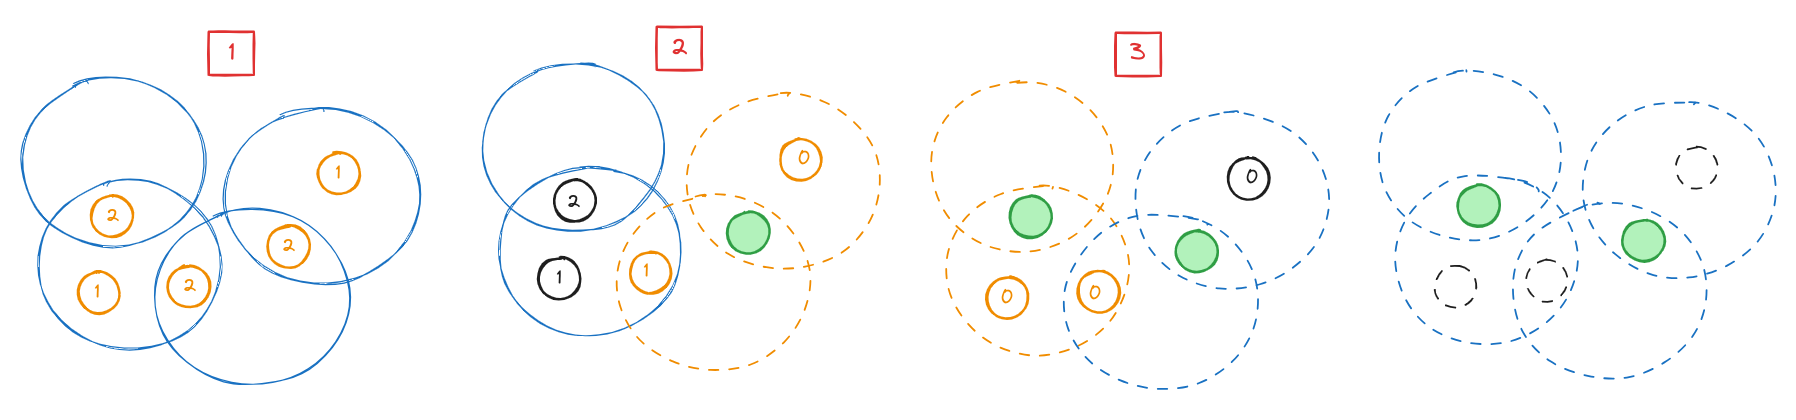
\includegraphics[width=0.8\textwidth]{img/greedy_ej2_mgr.png}
    \caption{Ejemplo 2 resuelto por Máximo global con recálculo}
    \label{fig:greedy_ej2_mgr}
\end{figure}

Por último, en el ejemplo de la fig. \ref{fig:greedy_ej3}, tanto "Máximo por grupo" (fig. \ref{fig:greedy_ej3_mpg}) como "Máximo global con recálculo" (fig. \ref{fig:greedy_ej3_mgr}) no llegan al la solución óptima.

\begin{figure}[H]
    \centering
    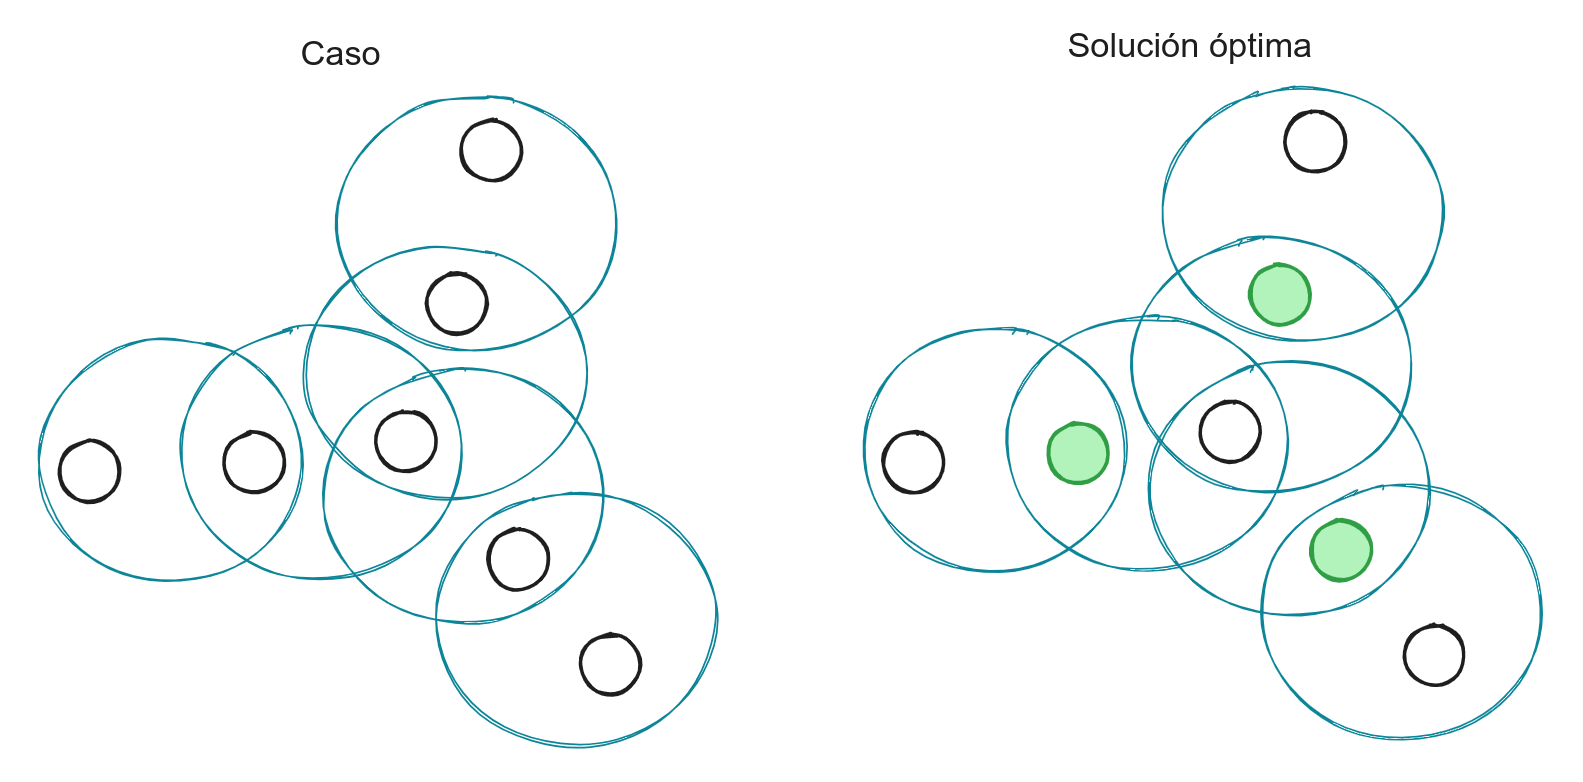
\includegraphics[width=0.8\textwidth]{img/greedy_ej3.png}
    \caption{Ejemplo 3}
    \label{fig:greedy_ej3}
\end{figure}

\begin{figure}[H]
    \centering
    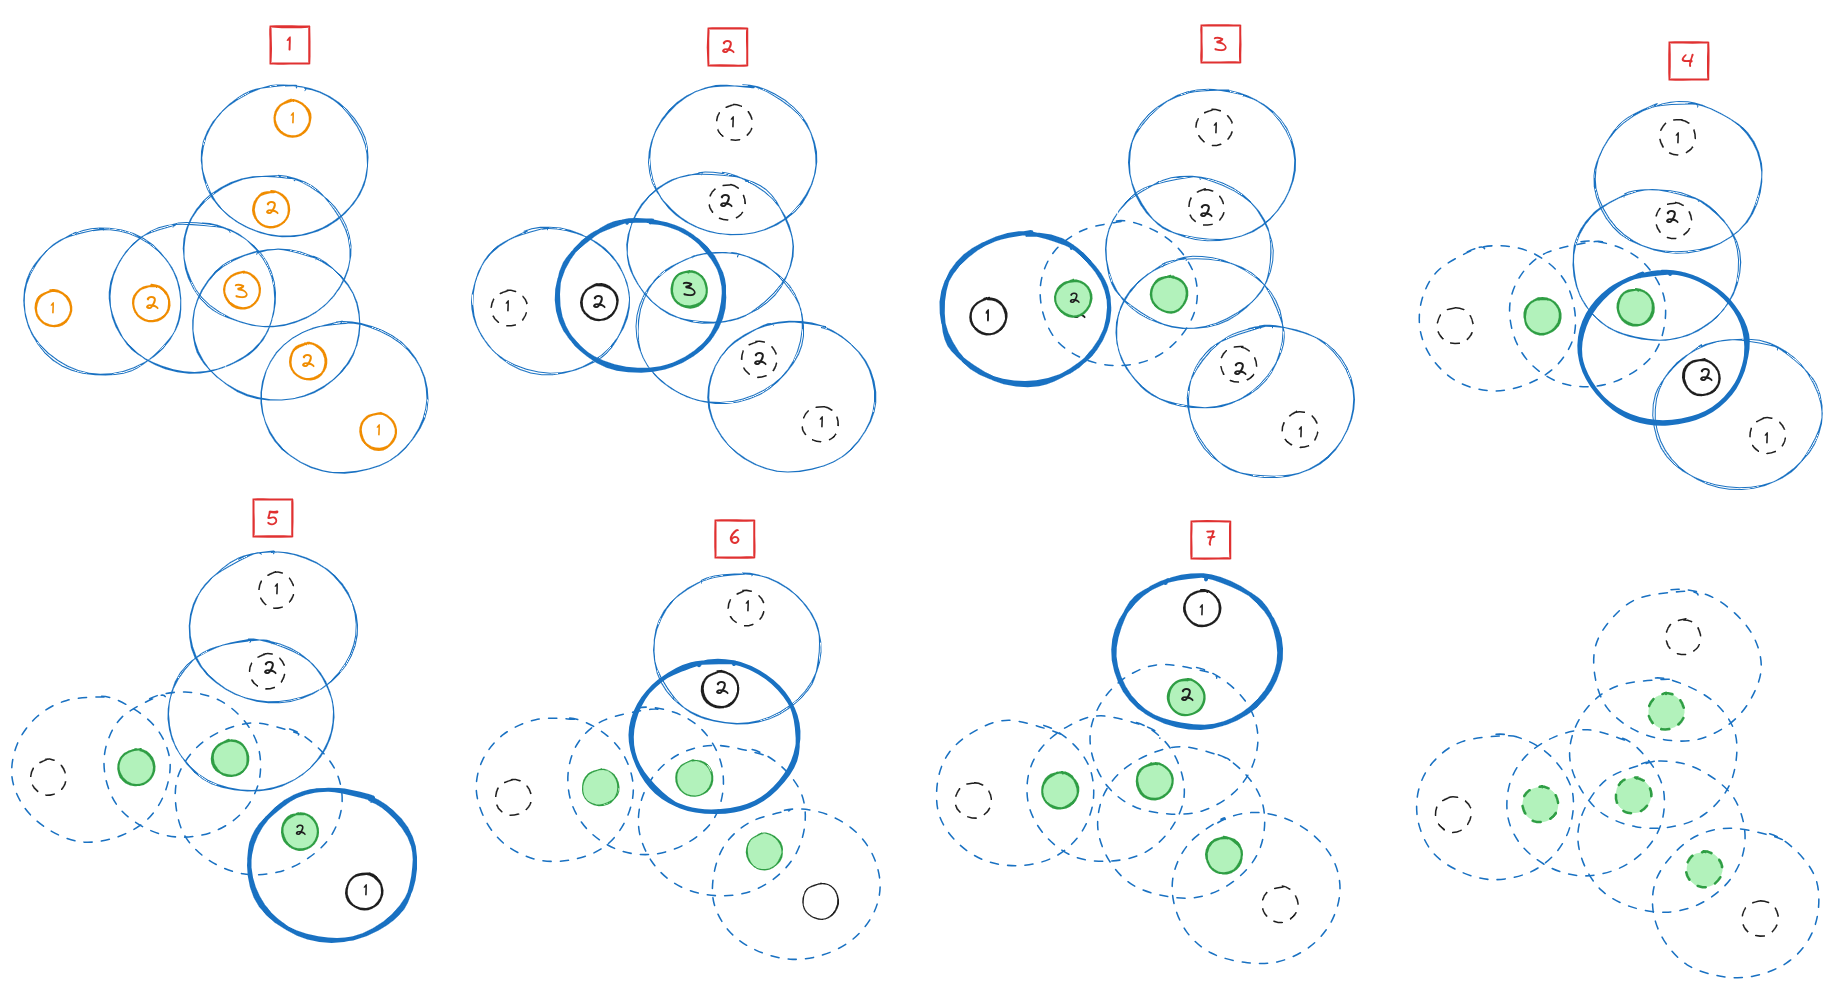
\includegraphics[width=0.8\textwidth]{img/greedy_ej3_mpg.png}
    \caption{Ejemplo 3 resuelto por Máximo por grupo}
    \label{fig:greedy_ej3_mpg}
\end{figure}

\begin{figure}[H]
    \centering
    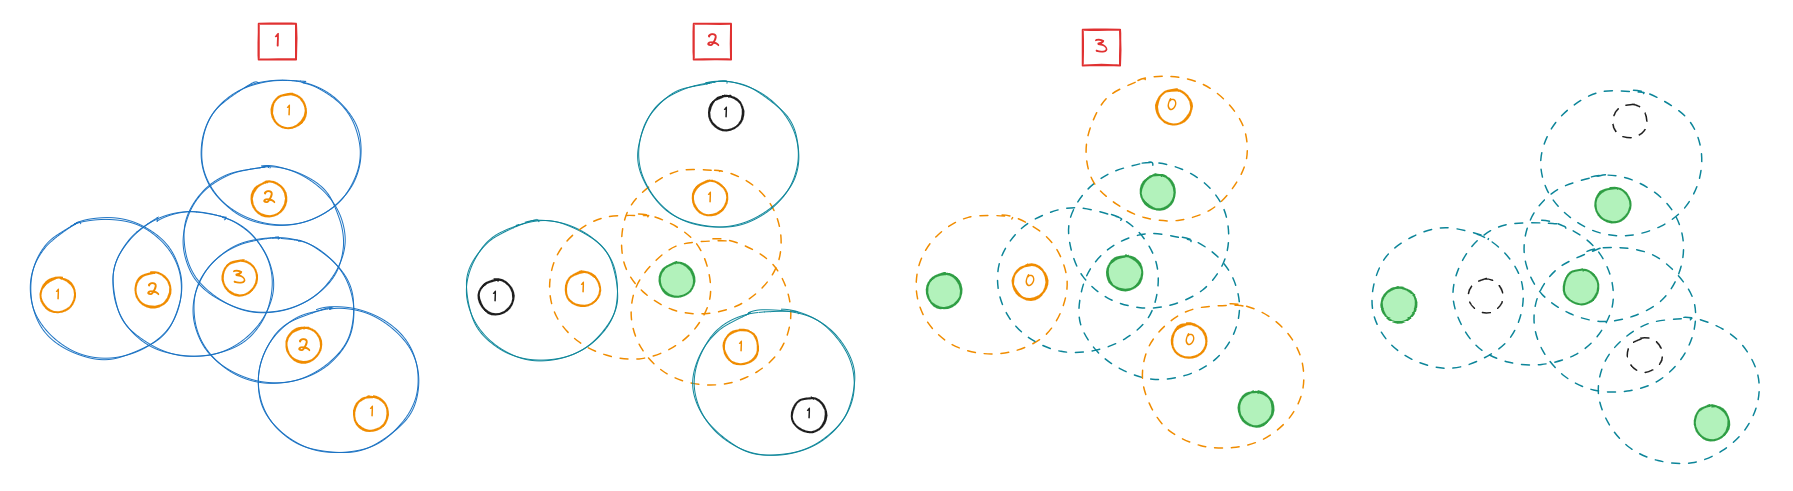
\includegraphics[width=0.8\textwidth]{img/greedy_ej3_mgr.png}
    \caption{Ejemplo 3 resuelto por Máximo global con recálculo}
    \label{fig:greedy_ej3_mgr}
\end{figure}